\section{Introduction}

In the previous chapters we discussed algorithms that operated on finite field elements as if they were made of individual bits (the binary coefficients). This is a sensible approach for building circuits, as the bits map naturally to simple signals, allowing the circuits to be constructed with basic logic gates. \\

However, during our research we also studied $GF(2^m)$ arithmetic for CPUs, where the individual bit approach is not efficient. In theory software could also operate on individual bits of each element, but this would require multiple instructions to process each bit, not to mention additional overhead on architecture incapable of addressing single bits. \\

On software implementations, the more sensible approach is to group the coefficients into CPU words (see Fig.~\ref{fig_simple_words}). Because this introduces a new layer of complexity, we decided to focus on the small but important area of polynomial reduction modulo a trinomial, a common operation in $\F_2[x]/(x^m+x^a+1)$. \\

\begin{figure}
  \caption{Representation of a binary field element with bits divided into words.}
  \label{fig:simple_words}
  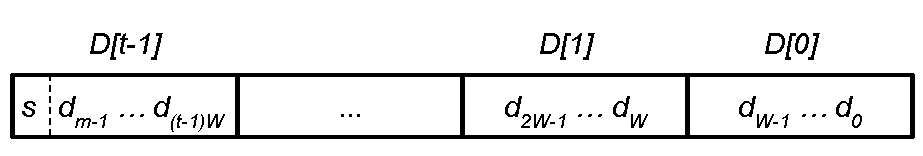
\includegraphics[width = .55\columnwidth]{figures/element-word.pdf}
\end{figure}

This operation has some important practical applications. Using a trinomial as irreducible polynomial is  preferred when available because it maximizes the number of zero coefficients in the the irreducible polynomial, enabling numerous simplifications. And the reduction operation is an important step for multiplications and exponentiations, making speedups desirable.

\section{Operating on words}\label{operating-on-words}

Manipulation of individual bits is not efficient in most CPU architectures. In general, it is preferred to operate on words, with a size specific to the microprocessor architecture, such as $32$- or $64$-bit words. However, the reduction algorithms are strongly bit oriented, since the coefficients are not naturally grouped in words. The codification of these algorithms to word oriented programming languages usually adds some complexity in terms of bitwise shifts and masks, and doesn't enjoy the parallelism inherent in XOR circuits. Specific techniques that help us in this coding have been proposed in the literature\cite{Hilewitz2008}. 

In this scenario it's often desirable to have "interoperability", choosing a field size and a irreducible polynomial that leads to efficient operations
in both hardware and software implementations. A straightforward
approach to this problem is to develop a hardware implementation first,
XOR'ing individual bits, and convert the algorithm to words. This can be
thought of as parallelizing the operations, with SHIFTs and AND/OR masks
for alignment. This is the approach used in this document.

The word-oriented algorithm can be helped by choosing specific field sizes and irreducible polynomials that introduce operations aligning at word boundaries, to avoid these bitwise shifts and masks, or that map well to architecture-specific operations. In our algorithms we try to make use of alignment opportunities when they appear, but do not depend on them or any specific architecture.

\section{Delay independence}

Performing binary polynomial reduction in a CPU has a few differences from implementing a hardware circuit. For example, circuits often avoid irreducible polynomials with the second largest exponent $a > \ceil{m/2}$. As seen before with pentanomials, this characteristic leads to higher delays in most circuit-based reduction algorithms. This is caused by the inter-dependency of the calculations, limiting the natural parallelism of circuits and thus increases the total delay.

This property does not affect software implementations. To illustrate this, we take two algorithms that perform modular reduction for the NIST irreducible trinomials $x^{233} + x^{74} + 1$ and $x^{409} + x^{87} + 1$~\cite[p. 55]{hankerson2006guide}. Then we manually adapt each of these algorithms to perform a reduction modulo its reciprocal, $x^m + x^{a-m} + 1$. Notice the only change required is in the indexing and bitwise shifts. The total number of operations remains the same. Algorithms meant for circuit implementations, on the other hand, would have different delay characteristics on each version. % Muito pouco. Expandir. Mostrar diferenças linha-a-linha.

% Explicar melhor os algoritmos.

% Exemplos de execução (olhar no livro do hankerson)

% Tabela comparando custo para deixar explícito que o custo é o mesmo.

\begin{algorithm}
\begin{algorithmic}[1]
  \REQUIRE $C[2m-2,0]$
  \ENSURE $C[m-1,0]$
  \FOR{$i \gets 15$ \textbf{downto} $8$}
    \STATE $T \gets C[i]$
    \STATE $C[i-8] \gets C[i-8] \oplus T << 23$
    \STATE $C[i-7] \gets C[i-7] \oplus T >> 9$
    \STATE $C[i-5] \gets C[i-5] \oplus T << 1$
    \STATE $C[i-4] \gets C[i-4] \oplus T >> 31$
  \ENDFOR
  \STATE $T \gets C[7] >> 9$
  \STATE $C[0] \gets C[0] \oplus T$
  \STATE $C[2] \gets C[2] \oplus T << 10$
  \STATE $C[3] \gets C[3] \oplus T >> 22$
  \STATE $C[7] \gets C[7] \& \texttt{0x1FF}$
  \RETURN $C$
  \caption{Hankerson's algorithm for reduction modulus $x^{233} + x^{74} + 1$, a standardized NIST polynomial.}
  \label{alg:233_74_nist}
\end{algorithmic}
\end{algorithm}

 \begin{algorithm}
 \begin{algorithmic}[1]
  \REQUIRE $C[2m-2,0]$
  \ENSURE $C[m-1,0]$
  \FOR{$i \gets 14$ \textbf{downto} $8$}
    \STATE $T \gets C[i]$
    \STATE $C[i-8] \gets C[i-8] \oplus T << 23$
    \STATE $C[i-7] \gets C[i-7] \oplus T >> 9$
    \STATE $C[i-3] \gets C[i-3] \oplus T << 22$
    \STATE $C[i-2] \gets C[i-2] \oplus T >> 10$
  \ENDFOR
  \STATE $T \gets C[7] >> 9$
  \STATE $C[0] \gets C[0] \oplus T$
  \STATE $C[2] \gets C[2] \oplus T << 31$
  \STATE $C[3] \gets C[3] \oplus T >> 1$
  \STATE $C[7] \gets C[7] \& \texttt{0x1FF}$
  \RETURN $C$
  \caption{Algorithm for reduction modulus $x^{233} + x^{159} + 1$, $(233, 74)$'s recriprocal.}
  \label{alg:233_159}
\end{algorithmic}
\end{algorithm}

\begin{algorithm}
\begin{algorithmic}[1]
  \REQUIRE $C[2m-2,0]$
  \ENSURE $C[m-1,0]$
  \FOR{$i \gets 25$ \textbf{downto} $13$}
    \STATE $T \gets C[i]$
    \STATE $C[i-13] \gets C[i-13] \oplus T << 7$
    \STATE $C[i-12] \gets C[i-12] \oplus T >> 25$
    \STATE $C[i-11] \gets C[i-11] \oplus T << 30$
    \STATE $C[i-10] \gets C[i-10] \oplus T >> 2$
  \ENDFOR
  \STATE $T \gets C[12] >> 25$
  \STATE $C[0] \gets C[0] \oplus T$
  \STATE $C[2] \gets C[2] \oplus T << 23$
  \STATE $C[12] \gets C[12] \& \texttt{0x1FFFFFF}$
  \RETURN $C$
  \caption{Hankerson's algorithm for reduction modulus $x^{409} + x^{87} + 1$, a standardized NIST polynomial.}
  \label{alg:409_87_nist}
\end{algorithmic}
\end{algorithm}


\begin{algorithm}
\begin{algorithmic}[1]
  \REQUIRE $C[2m-2,0]$
  \ENSURE $C[m-1,0]$
  \FOR{$i \gets 25$ \textbf{downto} $13$}
    \STATE $T \gets C[i]$
    \STATE $C[i-13] \gets C[i-13] \oplus T << 7$
    \STATE $C[i-12] \gets C[i-12] \oplus T >> 25$
    \STATE $C[i-3] \gets C[i-3] \oplus T << 9$
    \STATE $C[i-2] \gets C[i-2] \oplus T >> 23$
  \ENDFOR
  \STATE $T \gets C[12] >> 25$
  \STATE $C[0] \gets C[0] \oplus T$
  \STATE $C[10] \gets C[10] \oplus T << 2$
  \STATE $C[12] \gets C[12] \& \texttt{0x1FFFFFF}$
  \RETURN $C$
  \caption{Algorithm for reduction modulus $x^{409} + x^{322} + 1$, $(409, 87)$'s reciprocal.}
  \label{alg:409_322}
\end{algorithmic}
\end{algorithm}

\section{Notations}

In this paper, we assume that one word has $W$ bits where $W$ is a multiple of $8$. The bits of a word $A$ are numbered from $0$ to $W-1$, with the rightmost bit corresponding to the $x^0$ coefficient (LSB) of $A$ designated as bit $0$. The following standard notation is used to denote operations on words $A$ and $B$:\\

\begin{tabular}{ll}
  $A \BitXOR B$ & bitwise exclusive or. \\
  $A \BitOr B$ & bitwise or. \\
  $A \BitAnd B$     & bitwise $AND$. \\ 
  $A \ShiftLeft n$     & left shift of $A$ by $n$ positions, ($n<W$), with the bits from 0 to $n-1$ set to $0$. \\
  $A\ShiftRight n$    & righ shift of $A$ by $n$ positions, ($n<W$), with bits from $W-n$ to $W-1$ set to $0$. \\
  $a, b, c, d$ & Polynomials in $\F_2[x]$, not necessarily an element of the field $\F_{2^m}$ (they may be an intermediate result before the final reduction).\\
  $A, B, C, D$ & Vector of bits corresponding to the polynomials $a, b, c, d$.\\
\end{tabular}\\

\section{Bit grouping}

Figure~\ref{fig:elemento:field} shows the representation of a element $d \in \ftwom$ as an array $D$ of $t$ words of $W$ bits, where $t = \left \lceil \frac{m}{W} \right \rceil$. The $s = tW-m$ highest order bits of $D[t-1]$ are not unused.
\begin{figure}[htb]
  \centering
  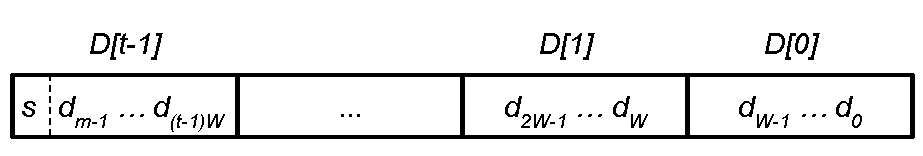
\includegraphics[width = .55\columnwidth]{figures/element-word.pdf}
\caption{Representation of $d \in \ftwom$ as an array $D$ of $W$ bit words. The $s = tW-m$ highest order bits of $D[t-1]$ are not unused.}
\label{fig:elemento:field}
\end{figure}
\\

For the case where $(m-1) \mod{W} > \frac{W}{2}$, the Figure~\ref{fig:elemento:field:mult} shows the representation of an element $d = ab$, $a,b \in \ftwom$ as an array $D$ of $W$-bit words. The $s = 2(tW-m)+1$ highest order bits of $D[2t-1]$ are not unused.

\begin{figure}[htb]
  \centering
  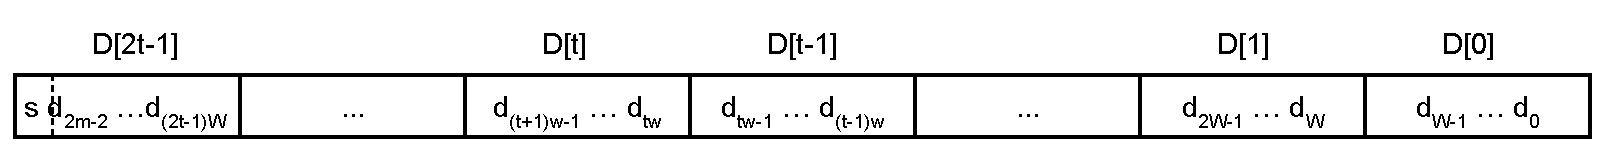
\includegraphics[width = .9\columnwidth]{figures/two-word-element-1.pdf}
\caption{Representation of $d = ab$, $a,b \in \ftwom$ as an array $D$ of $W$-bit words. The $s = 2(tW-m)+1$ highest order bits of $D[2t-1]$ are not unused.}
\label{fig:elemento:field:mult}
\end{figure}


When $(m-1) \mod{W} \leq \frac{W}{2}$, $D[2t-1]$ is not needed.  Figure~\ref{fig:elemento:field:mult2} shows the representation of a element $d = ab$, $a,b \in \ftwom$ as an array $D$ of $W$-bit words. The $s = 2(tW-m)+1$ highest order bits of $D[2t-2]$ and $D[2t-1]$ are not unused.
\begin{figure}[htb]
  \centering
  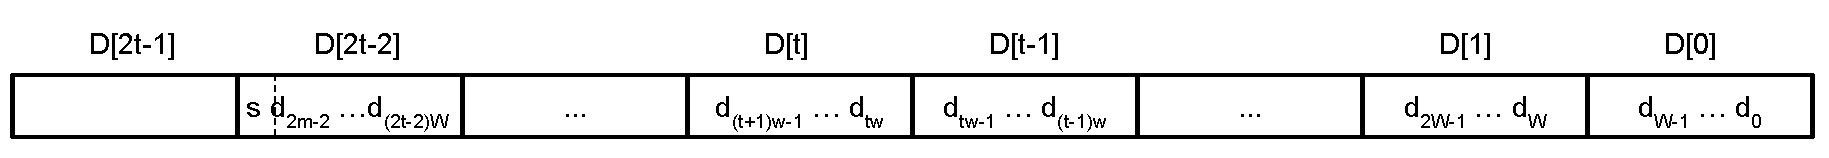
\includegraphics[width = \columnwidth]{figures/two-word-element-2.pdf}
\caption{Representation of $d = ab$, $a,b \in \ftwom$ as an array $D$ of $W$-bit words. The $s = 2(tW-m)+1$ highest order bits of $D[2t-2]$ and $D[2t-1]$ are not unused.}
\label{fig:elemento:field:mult2}
\end{figure}

In these cases a whole word is wasted, but length calculations become simpler: to get the length (in words) of a product of two elements, just add their lengths (in words).